% !TEX root = ../presentation.tex

\subsubsection[Simulation]{Simulation}
\begin{frame}
\frametitle{Numerical Example}

\begin{itemize}
\item True Attitude Trajectory
    \begin{center}
    \animategraphics[controls,autoplay,loop,width=0.5\textwidth, height=0.5\textheight,keepaspectratio]{8}{animation/3Dpend/3Dpend_}{1}{1958}
\end{center}
\pause
\item Measurement
	\begin{itemize}
	\item Angular velocity: $50\,\mathrm{Hz}$ with the mean error of $0.45\,\mathrm{rad/s}$
	\item Attitude: $10\,\mathrm{Hz}$ with the mean errr of $10.04^\circ$
	\end{itemize}
\end{itemize}


\end{frame}


\begin{frame}
\frametitle{Numerical Example}

\only<1>{
\begin{itemize}
\item Single matrix Fisher: \quad \Emph{large initial error} with $F(0)=100\exp (\pi\hat e_1)$
	\begin{itemize}
	\item Initial error: $180^\circ$, Initial singular values $s=100$
	\item \Emph{Falsely too confident} about the \Emph{completely wrong attitude}
	\end{itemize}
\end{itemize}


\begin{figure}\setcounter{subfigure}{0}
\centerline{
    \subcaptionbox{ Attitude estimation error ($\mathrm{deg}$) }[0.5\textwidth]{\hspace*{0.03\columnwidth}
		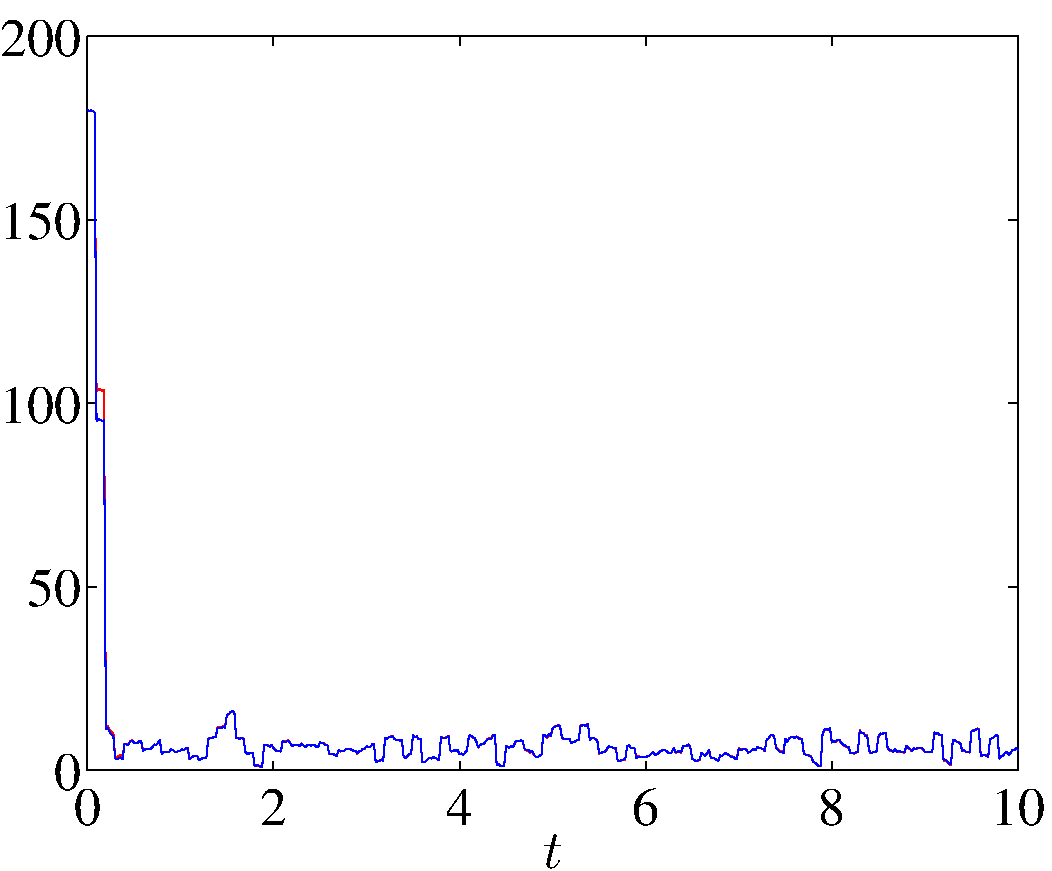
\includegraphics[height=0.6\textheight,width=0.5\textwidth,keepaspectratio]{figures/2017AAS_matrix_fisher/TAC16_0_R_est_err}\label{fig:R_est_err_0}\hspace*{0.03\columnwidth}}~
                \subcaptionbox{ Uncertainty measured by $\frac{1}{s_i+s_j}$ }[0.5\textwidth]{
		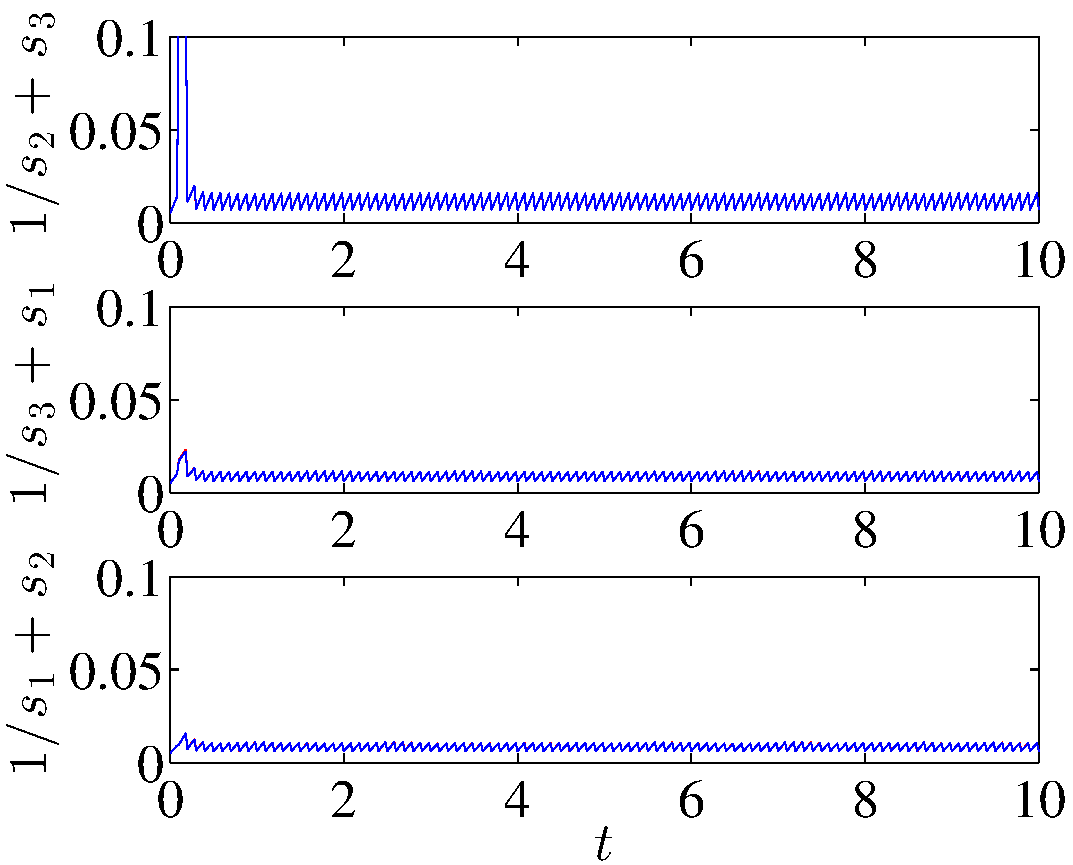
\includegraphics[height=0.6\textheight,width=0.5\textwidth,keepaspectratio]{figures/2017AAS_matrix_fisher/TAC16_0_s}}
}
\end{figure}}

\only<2>{
    \tiny
\begin{figure}
    \centering
    \subcaptionbox{ \tiny $t=0$,~$p_{\max}=1.45\times 10^4$ }[0.33\textwidth]{
        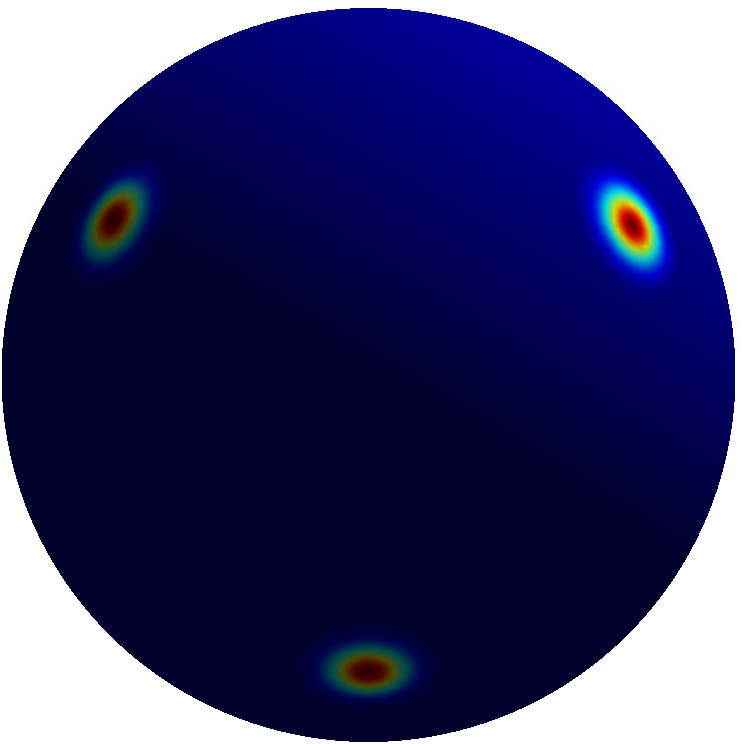
\includegraphics[width=0.4\textwidth,height=0.35\textheight,keepaspectratio]{figures/2017AAS_matrix_fisher/TAC16_0_F_1b}}~
    \subcaptionbox{ \tiny $t=0.08$, $p_{\max}=4.38\times 10^3$ }[0.33\textwidth]{
        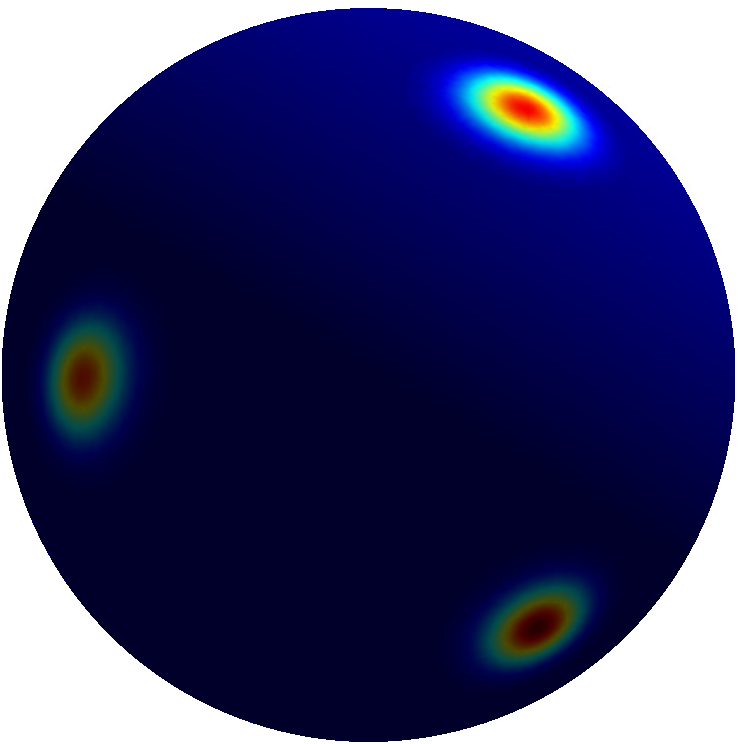
\includegraphics[width=0.33\textwidth,height=0.35\textheight,keepaspectratio]{figures/2017AAS_matrix_fisher/TAC16_0_F_5b}}~
    \subcaptionbox{ \tiny $t=0.1$, $p_{\max}=1.08\times 10^{3}$ }[0.33\textwidth]{
            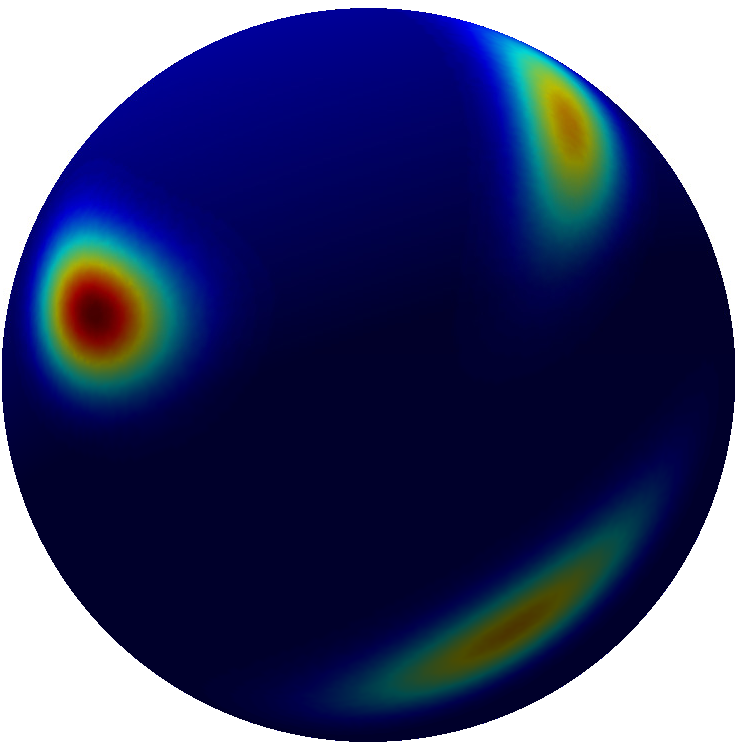
\includegraphics[width=0.33\textwidth, height=0.35\textheight, keepaspectratio]{figures/2017AAS_matrix_fisher/TAC16_0_F_6b}}\\
    \subcaptionbox{ \tiny $t=0.3$, $p_{\max}=8.73\times 10^3$ }[0.33\textwidth]{
        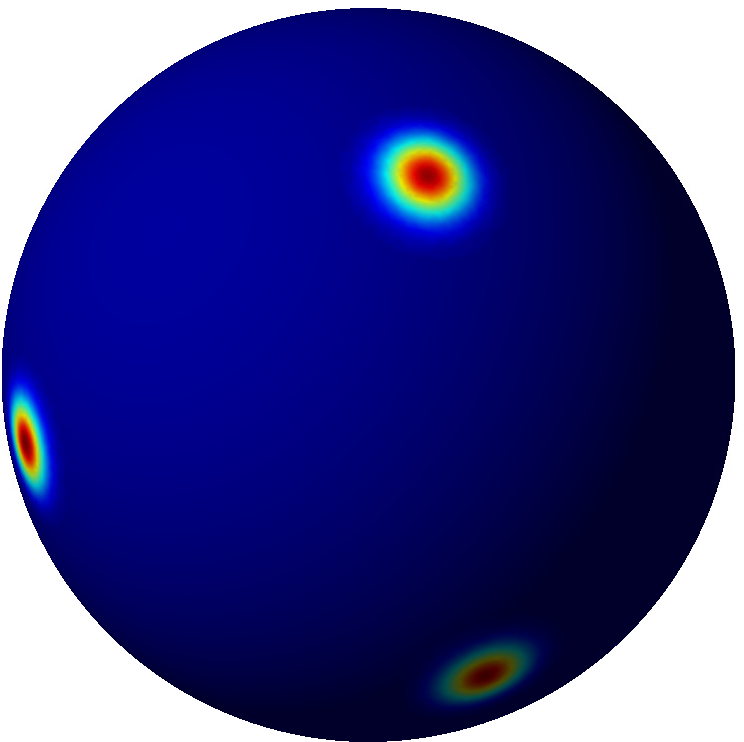
\includegraphics[width=0.33\textwidth,height=0.35\textheight,keepaspectratio]{figures/2017AAS_matrix_fisher/TAC16_0_F_16b}}~
    \subcaptionbox{\tiny $t=1$, $p_{\max}=9.61\times 10^3$ }[0.33\textwidth]{
        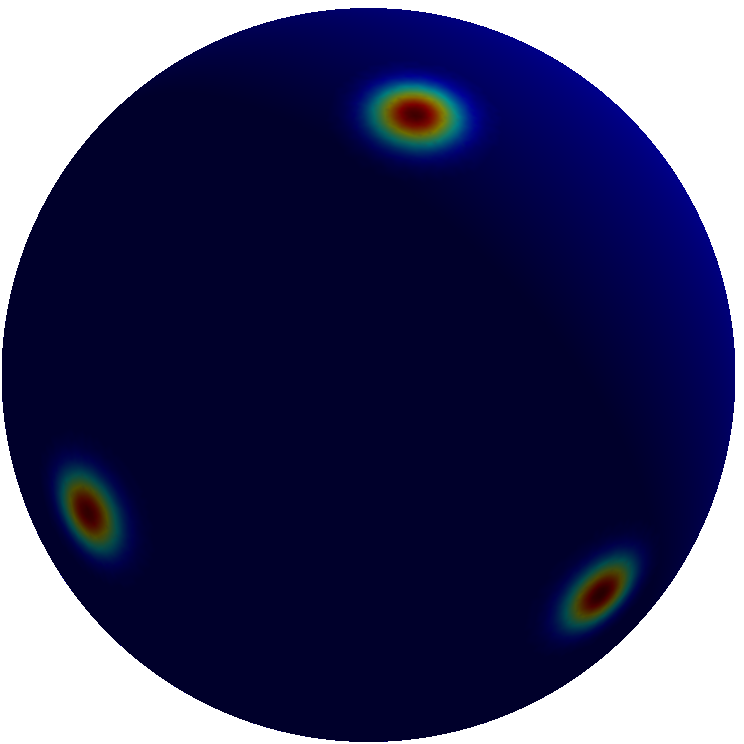
\includegraphics[width=0.33\textwidth,height=0.35\textheight,keepaspectratio]{figures/2017AAS_matrix_fisher/TAC16_0_F_51b}}~
    \subcaptionbox{\tiny $t=10$, $p_{\max}=9.82\times 10^3$ }[0.33\textwidth]{
        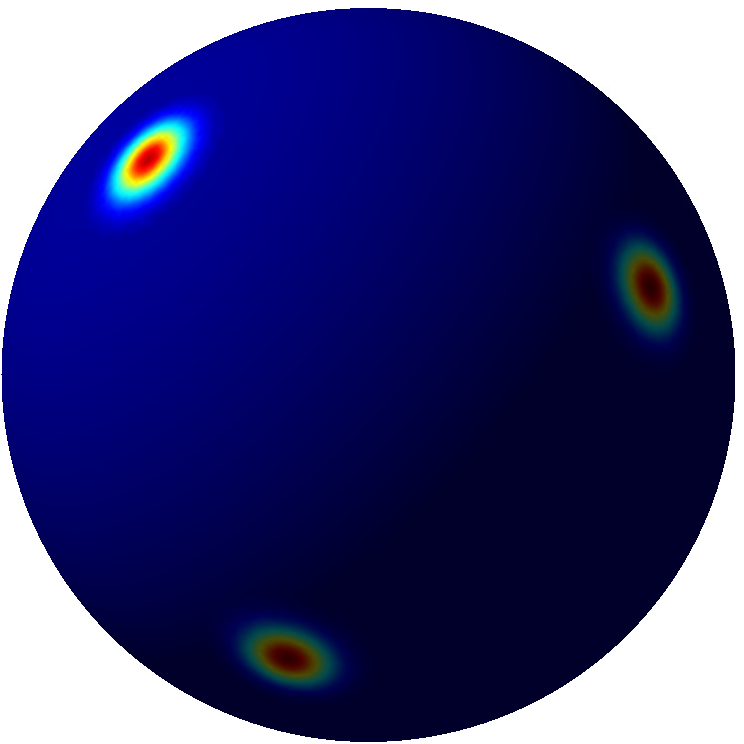
\includegraphics[width=0.33\textwidth,height=0.35\textheight,keepaspectratio]{figures/2017AAS_matrix_fisher/TAC16_0_F_501b}}
    \caption{Case I: visualizations of $\mathcal{M}(F_k)$ for the first-order filter}\label{fig:visES_0}
\end{figure}
}

\end{frame}

\begin{frame}
\frametitle{Numerical Example}

\only<1>{
\begin{itemize}
\item Matrix Fisher mixture: \Emph{large uncertainty} with three components
	\begin{itemize}
        \item True initial attitude: $R_{true}(0)=I_{3\times 3}$ and estimator is biased by three inaccurate estimates with large errors
	    \item Initially uncertain of rotation about first body fixed axis
	\end{itemize}
\end{itemize}

\begin{columns}
\begin{column}{0.5\textwidth}
    {\small
    \begin{gather*}
F_{1_0} = 20 \exp (\frac{1}{3}\pi\hat e_1),\quad \alpha_{1_0}=\frac{1}{4}, \\
F_{2_0} = 20 \exp (\frac{2}{3}\pi\hat e_1),\quad \alpha_{2_0}=\frac{1}{2}, \\
F_{3_0} = 20 \exp (\pi\hat e_1)\quad \alpha_{3_0}=\frac{1}{4}.
\end{gather*}}
\end{column}
\begin{column}{0.5\textwidth}
\begin{figure}\setcounter{subfigure}{0}
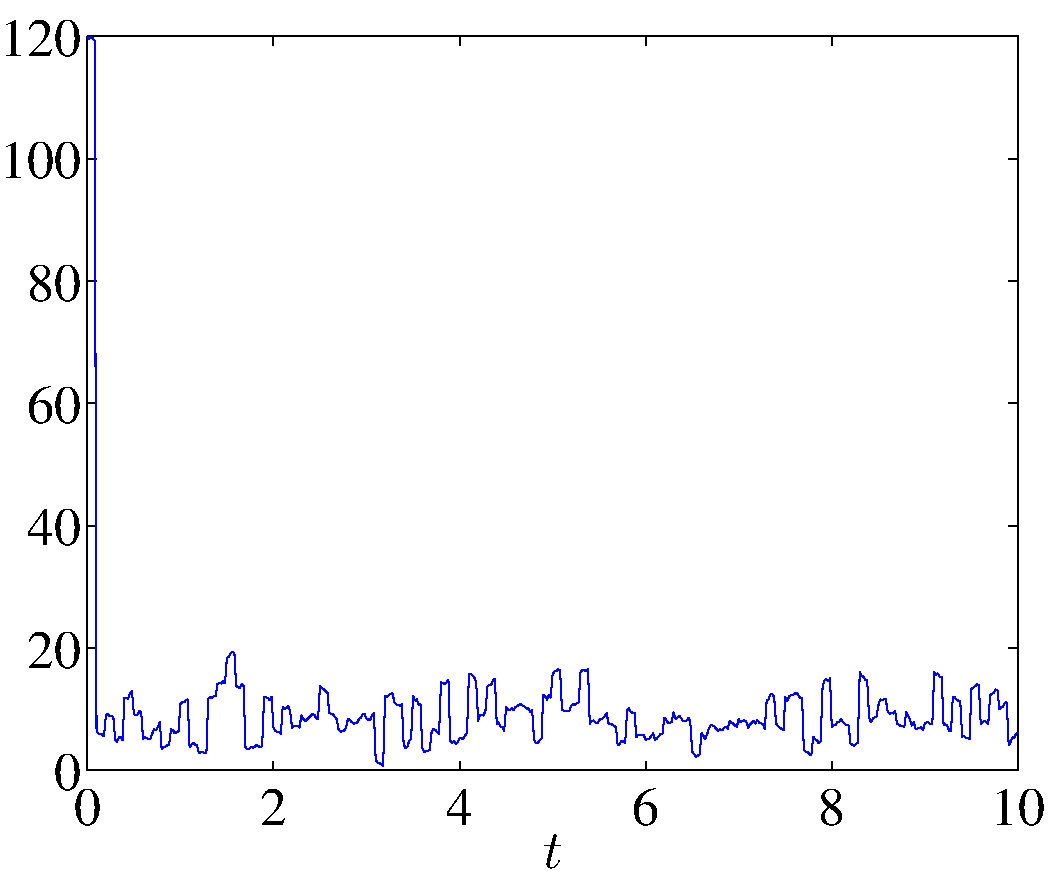
\includegraphics[width=\textwidth,height=0.65\textheight,keepaspectratio]{figures/2017AAS_matrix_fisher/AAS17_1_R_est_err} 
\end{figure}
\end{column}
\end{columns}
}

\only<2>{
\begin{figure}
	\subcaptionbox{ \tiny $t=0$, $p_{mse}=6.47\times 10^-7$ }[0.33\textwidth]{
		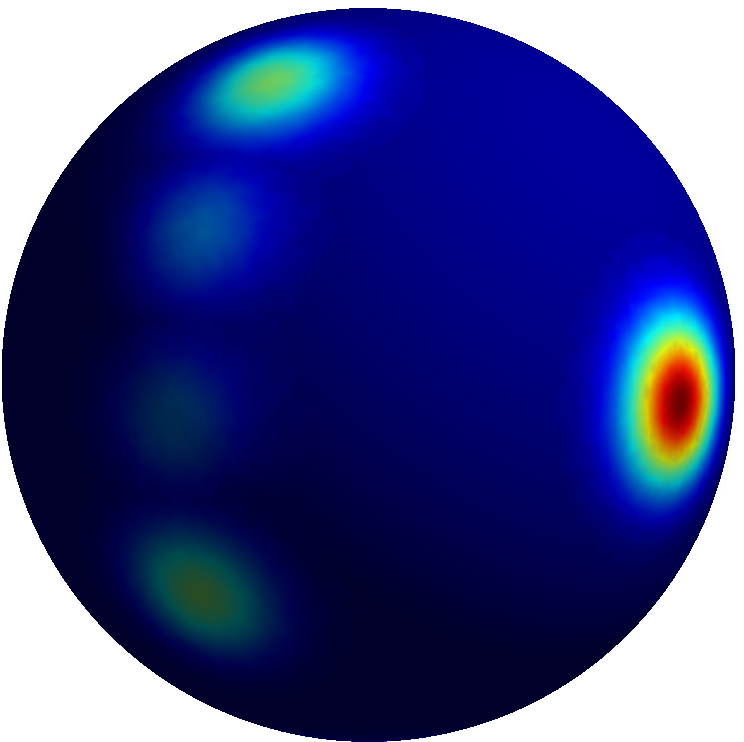
\includegraphics[width=0.33\textwidth,height=0.35\textheight,keepaspectratio]{figures/2017AAS_matrix_fisher/est_MF_mix_AAS17_1_1}}~
	\subcaptionbox{ \tiny $t=0.06$, $p_{mse}=3.4\times 10^-3$ }[0.33\textwidth]{
		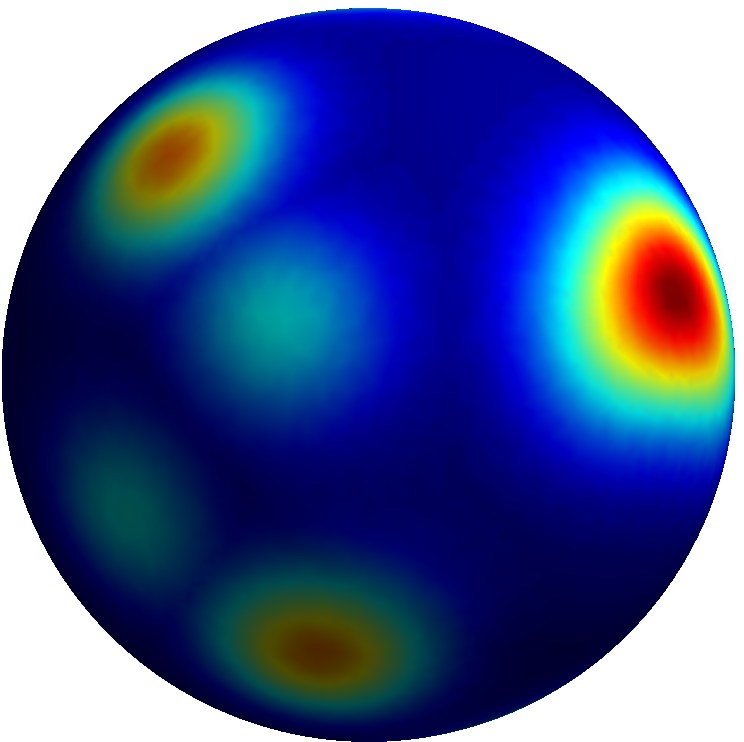
\includegraphics[width=0.33\textwidth,height=0.35\textheight,keepaspectratio]{figures/2017AAS_matrix_fisher/est_MF_mix_AAS17_1_4}}~
	\subcaptionbox{ \tiny $t=0.08$, $p_{mse}=4.2\times 10^{-3}$ }[0.33\textwidth]{
		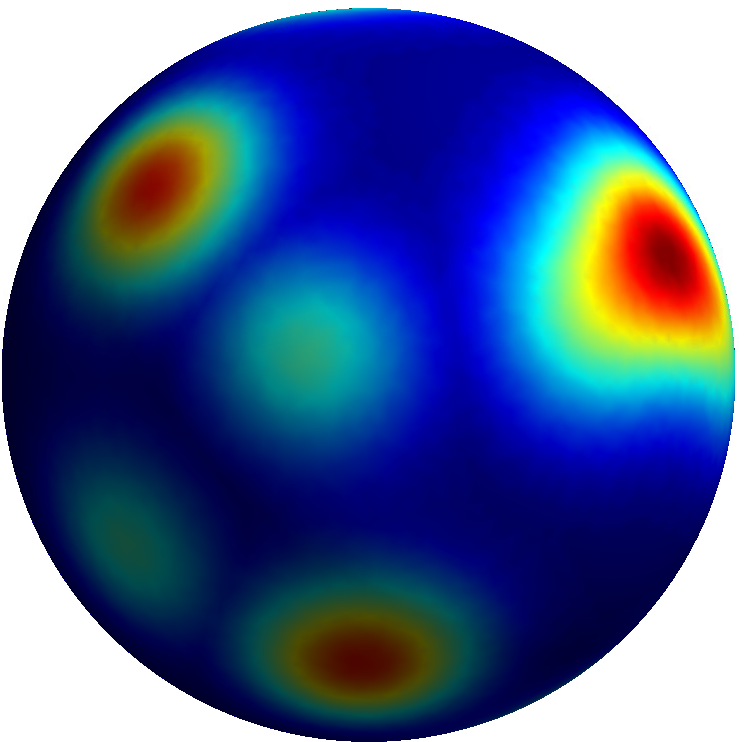
\includegraphics[width=0.33\textwidth,height=0.35\textheight,keepaspectratio]{figures/2017AAS_matrix_fisher/est_MF_mix_AAS17_1_5}}\\
	\subcaptionbox{ \tiny $t=0.1$, $p_{mse}=1.08\times 10^3$ }[0.33\textwidth]{
		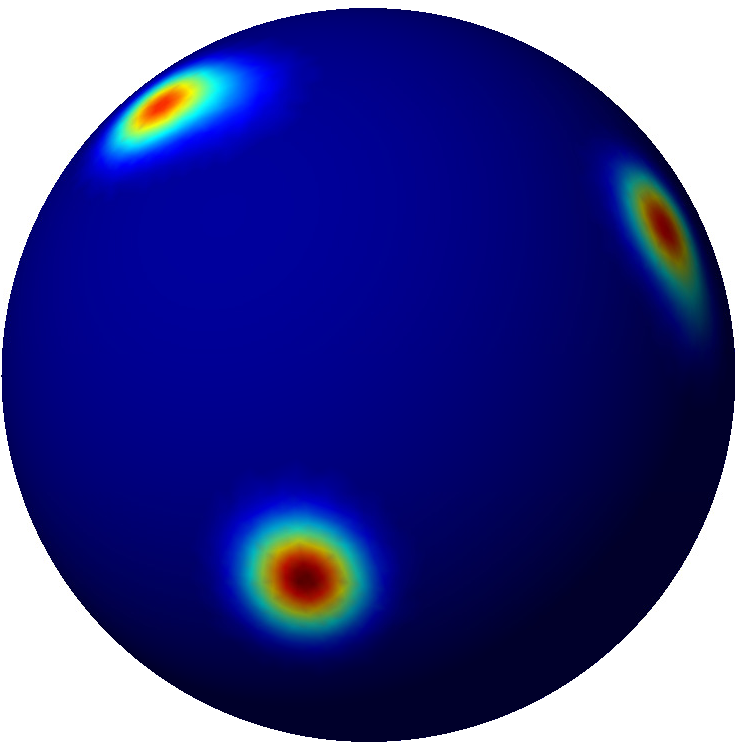
\includegraphics[width=0.33\textwidth,height=0.35\textheight,keepaspectratio]{figures/2017AAS_matrix_fisher/est_MF_mix_AAS17_1_6}}~
	\subcaptionbox{ \tiny $t=2$, $p_{mse}=1.29\times 10^3$ }[0.33\textwidth]{
		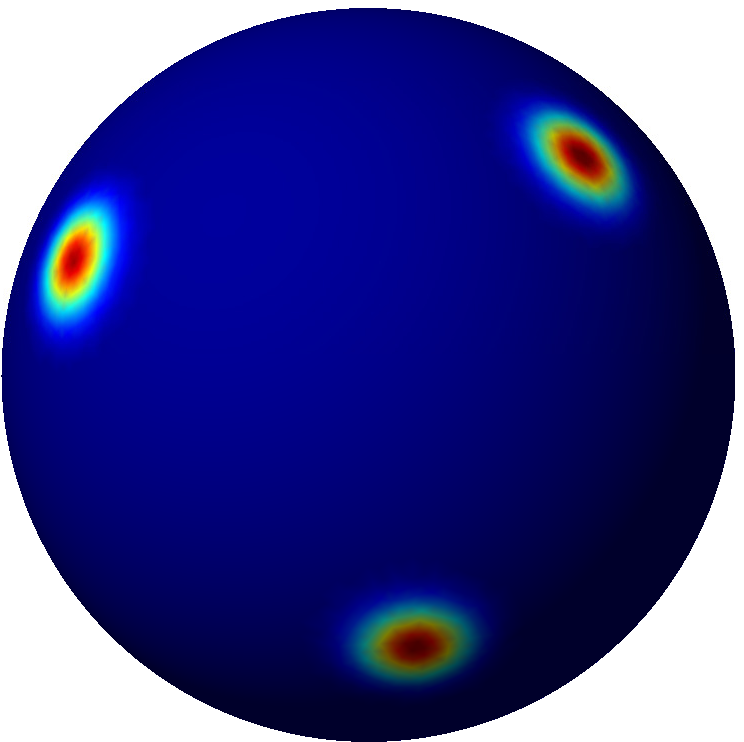
\includegraphics[width=0.33\textwidth,height=0.35\textheight,keepaspectratio]{figures/2017AAS_matrix_fisher/est_MF_mix_AAS17_1_11}}~
	\subcaptionbox{ \tiny $t=10$, $p_{mse}=1.29\times 10^3$ }[0.33\textwidth]{
		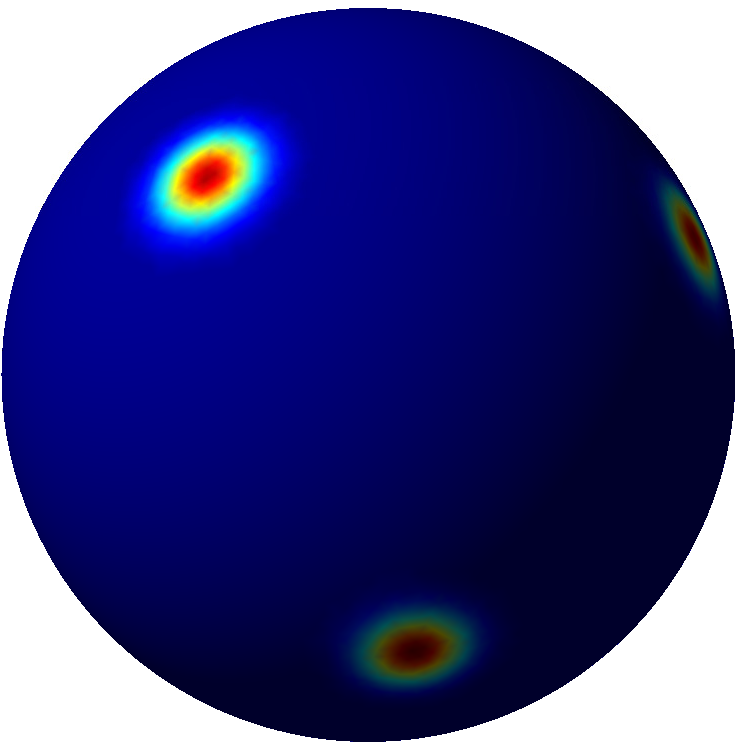
\includegraphics[width=0.33\textwidth,height=0.35\textheight,keepaspectratio]{figures/2017AAS_matrix_fisher/est_MF_mix_AAS17_1_501}}
\end{figure}
}

\end{frame}
